\chapter{Mining Transdiagnostics Symptoms in Social Media Data}
\section{Abstract}
Mining social media data to predict mental health condition and psychological traits have increasingly attracted attention in the clinical psychology domain. Instead of predicting a specific diagnosis criteria, we adopt a transdiagnostic approach by investigating common symptoms that  predispose an individual to a variety of mental disorders. Treatments that targets these factors are called transdiagnostic treatment, which has been widely employed to tackle anxiety and depression disorders.  We leverage FB data from 77 users who participated in the myPersonality project back in 2011.  We label negative emotion and two transdiagnositc components - reasoning bias (cognitive distortion) and negative thinking among more than 4000 Facebook posts. Our study includes how transdiagnostic symptoms manifested in users with different characteristics. We find that martial status and user's parental relationship are protective factors. Finally, we also identified language features that predict transdiagnotics symptoms.


\section{Introduction}
In the recent years, there is a surging amount of studies attempting to use social media data to predict psychopathology diagnosis. Various attempts on predicting depression has achieved good performance \cite{munmun13, Aldarwish17, Hu17, Coppersmith15}. What makes these prediction tasks challenging at the moment is comorbidity is very common in psychopathology. According to the literature, about 60\% - 70\% of individuals diagnosed with anxiety disorder also meet some of the criteria in depressive and affective disorders \cite{Timothy95}.

The traditional conceptual structure approach to understand psychological disorder is to provide a diagnosis of a specific disorder. However, there is increasing recognition that criteria diagnosis are of less value because many disorders frequently co-occurred and share a number of vulnerability factors, which is also called comorbidity \cite{Kessler98,Hirschfeld99}. In light of the challenge, psychologists are shifting towards a transdiagnositc approach in the recent years. Instead of giving multiple diagnosis to a patient with comorbidity, transdiagnostic approach focuses on common psychological processes underlie the syndromes, which provides a better explanation to the high rate of comorbidity observed in clinical practice \cite{Harvey04}. Treatments and preventative interventions targeting transdiagnostic symptoms have been found to effective among anxiety, depressive disorders \cite{Collins09,Norton04}, eating disorder \cite{Fairburn03} and social phobia \cite{Freda00}, etc. In support of transdiagnostic theory, the National Institute of Mental Health (NIMH), created the RDoC, The RDoc conceptualized five systems that underlie psychopathology: negative valence systems, positive valence systems, cognitive systems, systems for social processes and arousal/regulatory systems (Insel et al. 2010). 

The processes of producing language and the way language being used is an important aspect to identify psychopathology (Pennebeker). The cognitive system captures language as a contruct (Maria's paper), however, at present, analyzing language within the transdiagnostic approach framework hasn't been incorporated into analyzing social media data. In this paper, we see how the transdiagnostic symptoms identified from social media text contribute to depression, influence satisfaction with life and how it related to personality. Meanwhile, we also look at user characteristics that might contribute to some of the transdiagnostic symptoms. 

% Head 1
\subsection{Investigate Transdiagnositic Symptoms on Social Media}
We explore some of the transdiagnostic symptoms in social media posts. Social media users' threads and updates often reveal their opinions, emotions and daily life activities. Data capturing these information provide researchers a platform to study their behaviors and psychological traits \cite{Kosinski13, Lushi}. Motivated by the fact that most of the studies look at whether social media behaviors reflect mental health symptoms focus on a specific diagnosis criteria \cite{munmun13, Aldarwish17, Hu17, Coppersmith15}, which did not consider high comorbidity rate in many disorders. We consider to look at whether social media posts capture some of the transdiagnostics symptoms.

The components of transdiagnostic treatment or research include attention, memory, reasoning, thought and behaviour. Reasoning refers to thinking that involves deducing conclusions, generating judgements and testing hypotheses logically. Biased reasoning, which is in parallel with cognitive distortion in cognitive behavior therapy, often draws in conclusion different from the reality \cite{Harvey04}. Assessing cognitive distortion is an index of the improvements in behaviours and emotional resiliency \cite{Freda00,Neil96}.  Later we will explain the details of identifying cognitive distortion.

Another transdiagnostic component captured by social media text is repetitive negative thinking, which presents across affective disorders, anxiety disorders, insomnia or psychosis \cite{Harvey04}. The two processes in repetitive negative thinking are worry and rumination. They all share three commonalities: a) repetitive, b) uncontrollable c) focus on negative content \cite{Harvey04}. Worry presents mainly in general anxiety disorder (GAD),  which is defined as a chain of uncontrollable thoughts or images which represent an attempt to problem-solving an issue that might contains a negative outcome \cite{Thomas83}. Whereas, rumination are content specific to the type of disorder. Rumination on post traumatic stress disorder involves repetitive negative thinking about the trauma and its consequences \cite{Michael07}; Rumination in social phobia contains self-appraisals and evaluation of the partner in a social event \cite{Kashdan07}. 


\section{BACKGROUND AND RELATED WORK}
% Head 1
\subsection{The Cognitive Behavior Therapy (CBT)}

Cognitive models of psychopathology proposed that pathological behaviors and emotions are often the consequences of cognitive biases or distortion, which are inadequate interpretation of situations. Beck's cognitive model of psychopathology emphasizes the role of cognitive distortion in the the maintenance of anxiety, depression and other mental disorders \cite{Beck67,Beck11}. Therefore, one of the goals from cognitive behavioral therapy for anxiety and depression is to help an individual to adjust these biases, which is called “cognitive restructuring’.  Cognitive restructuring modifies the clients' problematic ways of thinking about themselves, their world and their future \cite{Harvey04}. To identify these biases, therapists observe thoughts contain cognitive distortions and investigate the underlying schema that generate the these thoughts \cite{Beck11,Dobson09}. 

Cognitive distortions can be classified according to its content. For example, mind reading, personalization, labeling and all-or-nothing thinking, etc. \cite{Oliveira14}. These thoughts can be true or dismissive to the reality. For example, "My boyfriend doesn't like me anymore." This statement may be true to the fact or based on mind reading, a type of distortion that refers to individuals assume that they know what people think without having sufficient evidence of their thoughts. The categories of cognitive distortions often indicate the type of disorder. For instance, individuals with social anxiety disorder engages in mind reading “No one wants me to be around with them” or catastrophizing "It will be a disaster if I said something wrong in the group".  Depressed individuals engages in a wide range of cognitive distortions - labeling "I am the black sheep of the family", fortune telling "I can never be happy without you" \cite{Newman15}. 

% Head 2
\subsection{Assessment of Cognitive Distortion}

The most widely applied method for assessing cognitive distortion is the cognitive distortion checklist. The list has been validated in experimental and clinical work \cite{Beck11,Dobson09}. xx and colleagues developed the Cognitive Distortion Questionnaire(CD-Quest) \cite{Simona17}, which is a 15-item questionnaire based on the distortion checklist that assess the frequency and intensity of cognitive distortion. It is administered before the therapy session to help a client to keep track on their thinking errors thus enabling them to be aware of the change over time as the therapy goes on. In this study, we adopted the CD-Quest in our annotation guideline as a criteria for annotators to identify cognitive distortion based on the context information provided in the Facebook posts. Below is an example from CD-Quest:

% quote
\begin{quote}
\textit{Dichotomous thinking (also called all-or-nothing, black-and-white, or
polarized thinking): I view a situation, a person, or an event in "either-or"
terms, fitting them into only two extreme categories instead of on a continuum.
EXAMPLES: "I made a mistake; therefore my performance was a failure." "I ate
more than I planned, so I blew my diet completely."}
\end{quote}

% Head 3
\subsection{Negative Emotion and Psychopathology}

The relationship between negative affect, depression and anxiety has been considered as clinically important historically (Akiskal, 1985; Clark, 1989; Clark and Watson, 1990; Dobson, 1985). How people react towards events tells their coping mechanism, at the heart of reacting and coping with events is people's emotional response (Pennebeker). We also investigate users' negative emotion on social media text and its correlation with user characteristics, behaviors and psychopathology. Instead of using LIWC, we manually label whether a post reflects negative emotion of the author. 

\section{Method and Materials}
% Head 1
\subsection{Data}
This corpus consists of 5000 Facebook posts from individuals who participated in the myPersonality project from January 2009 to December 2011. Our methods were carried out in accordance with the approved guidelines from myPersonality. myPersonality was a Facebook-based application collecting psychometric tests from users. Participants opt to allow myPersonality to collect their account information and public Facebook posts. collection of myPersonality complied with the terms of Facebook service. All data are anonymized and gathered with opt-in consents for research purposes. The sample used in our study contains 301 participants who have completed the CES-D scale, Satisfaction with Life Scale, Big-5 Personality Scale and Schwartz Value Survey. 

% Head 2
\subsection{Sampling Approach}
To ensure we have enough posts to conduct a longitudinal study. We only include regular posters in our sample. We define regular posters as individuals who posted twice per week or more. We estimated this using the average post count per day during the sampling frame. If an individual had a post count per day of 0.3, this individual made around 109.5 posts in 365 days, which was roughly equivalent to an average of 2.1057692 posts per week. In our sample, 122 out of 301 participants were regular posters. To make sure our sampling approach was conducted under a standard sampling framework, we included 91 regular posters whose last post obtained by myPersonality was less than a week before they completed the CES-D scale. Then we  obtain a sample of 4696 posts that were produced two months before CES-D score was obtained.  We future eliminate 14 posters who produced less than 20 posts during the two months and posts that are not written in English. Eventually we yield a sample of 4145 posts from 77 users. 

% Head 2
\subsection{Annotation Process}

The annotation guideline was developed using 4362 Facebook posts to illustrate negative emotion and cognitive distortions.  The extracted posts were first annotated by a specific trained psychologist according to the annotation guideline. The annotation process include three steps. First, we identify whether the post reflect the author's negative emotion, posts that contain a mixed of emotion is labeled as 'mixed'. We group the 'mixed' posts together with the negative emotion posts in the later analysis. Here negative emotion include but not limited to sadness, anger, anxious, boredom, physical complain and so on. Sometimes users repost content that contains negative emotion, but might not reflect negative emotion of the authors.  For example, 

% quote
\begin{quote}{\itshape}
\textit{you have a sister who has made you laugh, punched you, stuck up for you, drove you crazy, hugged you, watched you succeed , saw you fail, picked you back up, cheered you on, made you strong, and is someone you cant live without  someone you can always count on....REPOST THIS IF YOU HAVE A SISTER THAT YOU LOVE.}
\end{quote}

We label these posts as neutral because it is uncertain about the author's emotion when they repost this information. Second, we label posts that contain cognitive distortion. In scoring the cognitive distortion, annotators are given specific cues - CD-Quest as reference of the measurement of cognitive distortion, but are also instructed to rely on their linguistic intuition. In addition, posts from quotes, lyrics, and repost are labeled as non-original posts.  Annotators are trained by following instructions and sets of practice examples on the annotation guideline. The difficulty of this task is that a lot of the status contain emotion or thought but does not describe the event that cause the emotion or thought. However, we can still tell that some of the posts contain cognitive distortion even if the post doesn't indicate a situation or context, see table~\ref{tab:zero}. 

% Table
\begin{table}%
\caption{Posts with Dognitive distortion}
\label{tab:zero}
\begin{minipage}{\columnwidth}
\begin{center}
\begin{tabular}{|p{5cm}|p{9.5cm}|}
  \toprule
         post	& cognitive distortion   \\ 

  \hline\hline
  "I feel like my life is waste. I have no story, no influence, no particular skills that are useful. I just suck."
 & Labeling,magnification/minimization: The author assigns global negative traits to him/herself, such as 'my life is a waste',  'I just suck'. The author generate the global negative pattern based on some incidents, it is unsure the number of incident. But the author fail to focus on life events that are counter to this statement.  \\[5pt]
 \hline
  I hate the past. It deserves to be erased from memory forever. I don't care if the memories were good  &    Discounting positives and dichotomous thinking: the author hates everything in the past, which is all-or-nothing thinking and he/she diminishes the positive events or achievements in the past  \\[5pt]
  \hline
Nothing feels right today. It's weird  & The author gives greater weight to perceived failure or weakness but fail to aware of positive events or opportunities  \\[5pt]
  \bottomrule
\end{tabular}
\end{center}
\bigskip\centering

 \emph{Note:} 
\end{minipage}
\end{table}%

For the last step, we label posts that contain 
ffd- worry and rumination. Worry is often indicated by particular words, such as "anxious" and "nervous". Rumination includes ruminating on a specific event, state or emotion. Here we set the rumination time window as one week, if an individual ruminate on a specific event or a specific emotion/state within a week, we label it as rumination. However, rumination of a specific emotion could be difficult to identify if the post does not contain information about the event or situation that causes the emotion, because we cannot tell whether the negative emotion is pointed at the same event (see Example EMOTION).

% quote
\begin{quote}{\itshape}
EVENT: \\
\textit{"Cry my betts fish died and the other ones dying:("\\
"booh im crying my Betta fish died"}\\

STATE:\\
\textit{Ugh! What a boring morning!\\
I am so bored!\\
Why........SO..BOOOOOOOOOOOOOOOOOOOOREEEED!\\}

EMOTION: \\
\textit{Day1: "I'm so angry that mom threw away my things today." \\
Day 2: ":( "  \\
Day 3: ":(" } \\
\end{quote}

% Head 3
\subsection{Self-reported measurement scale}
We now present a number of user characteristics and three self-reported scales that are used to measure depression symptoms, personality ans satisfaction with life. Later we will investigate the relationships between and transdiagnostic symptoms and the self-reported psychological traits. 

\subsubsection{Center for Epidemiologic Studies Depression Scale (CES-D Scale)}
CES-D is a self-reported scale designed to measure depression symptoms in the general population\cite{Radloff77}. The scale consists of 20 depression symptoms associated items. It has been tested in psychiatric settings across various cultures over the years. It was found to have high internal consistency and test-retest reliability \cite{Radloff77,Herz86,Roberts80}. Its validity was assessed via correlation with clinical diagnosis of depression and other self-reported trait measurement \cite{Herz86}. 

\subsubsection{Five Factor Model of Personality (Big-5)}
The five factor personality model was established in an attempt to understand the description of traits. The dimensions composing the 5-factor models are extraversion, agreeableness, conscientiousness, neuroticism and openness to experience.  The five factor structure has been proved to be robust in both self and peer ratings \cite{McCrae92}, children and adult \cite{Ivan95} and across different cultures
\cite{McCrae02}. Early literature found that big-5 is relatively stable over time \cite{McCrae92}. However, recently literature found the opposite \cite{Ardelt00}. Neuroticism was found to have strong correlation with a bunch of psychological disorders, such as anxiety and depression \cite{Ormel04}. Individuals who score high on neuroticism tend to experience negative mood frequently and physical symptoms. Recent studies found that social media data can predict the 5-factor model of personality \cite{Kosinski13}. 

\subsubsection{Satisfaction with Life Scale (SWLS)}
The 5-item satisfaction with life scale was developed to measure global life satisfaction. The SWLS has been tested across different cultures and age groups \cite{Diener93} and has been found to have high internal consistency and temporal reliability \cite{Diener85}. Its validity was assessed by correlation with other measures of subjective well-being and specific personality dimension.

\section{Results}
% Head 1
\subsection{Transdiagnostic labels}
Among 4145 posts, 804 of them reflect negative emotion of the author, 36 of them contain a mix of positive and negative emotion. Among 840 posts that contain negative emotion, only 41 contain cognitive distortion, 111 contain negative thinking (85 worry, 26 rumination). 3 posts show both cognitive distortion and negative thinking. Cognitive distortion is rare, it only occurs in 1\% of the posts in this sample. We aggregate a negative emotion score by summing up the number of negative post from each user. We use the same approach to generate a distortion score and negative thinking score for each user. Table~\ref{tab:one} shows the statistics of the three scores  and their correlation with depression symptoms (CES-D). Table~\ref{tab:one2} shows the correlation between per post transdiagnostic symptom score with depression symptoms. It is appear that the cumulative transdiagnostic score is more strongly correlated with psychopathology. Therefore, we use the cumulative score in the later analysis. Although posts contain cognitive distortion only account for 1\% of all the posts but they are moderately correlated with self-depression symptoms. Whereas, negative emotion and negative thinking, although more frequently observed in the data, are not significantly correlated with CES-D.


% Table
\begin{table}%
\caption{Transdiagnositc components (cumulative score) and depression symptoms}
\label{tab:one}
\begin{minipage}{\columnwidth}
\begin{center}
\begin{tabular}{lllll}
  \toprule
        & mean	& SD   & CES-D & SWL \\ 
  \hline\hline
  Negative emotion  & 10.91 & 11.835 &0.192 & -0.16\\
  Cognitive distortion  & 0.532 & 0.981 &0.300** & -0.250* \\
  Negative thinking  & 1.441 & 2.962 &0.117& 0.023\\

  \bottomrule
\end{tabular}
\end{center}
\bigskip\centering

 \emph{Note:} * p<0.05, **p<0.01, ***p<0.001
\end{minipage}
\end{table}%

% Table
\begin{table}%
\caption{Transdiagnositc components (per post) and depression symptoms}
\label{tab:one2}
\begin{minipage}{\columnwidth}
\begin{center}
\begin{tabular}{lllll}
  \toprule
        & mean	& SD   &  CES-D  & SWL\\ 
  \hline\hline
  Negative emotion  & 0.182 & 0.197 &0.123 & -0.108\\
  Cognitive distortion  & 0.009 & 0.016 &0.261*& -0.208\\
  Negative thinking  & 0.018 & 0.032 &0.044 & -0.056\\

  \bottomrule
\end{tabular}
\end{center}
\bigskip\centering

 \emph{Note:} * p<0.05, **p<0.01, ***p<0.001, CES-D: correlation with depression symptoms. SWL: correlation with Satisfaction with Life
\end{minipage}
\end{table}%


Figure ~\ref{fig:one} shows the number of negative emotion and transdiagnostic symptom posts from each user in the two months time window. All the three distributions are negatively skew, which means most of the users do not have a lot of negative emotion, and a majority of the users do not show any cognitive distortion or negative thinking.  For those who shows cognitive distortion in their posts, they only have 1-2 posts shows cognitive distortion. 

% Figure
\begin{figure}`'
  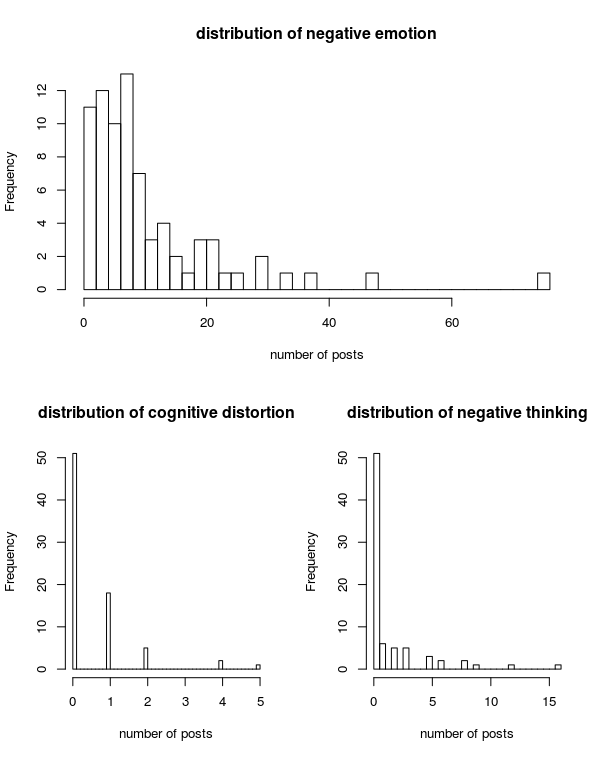
\includegraphics[width=80mm,scale=0.8]{fig1}
  \caption{Distribution of negative emotion and transdiagnostic symptoms}
  \label{fig:one}
\end{figure}

% Head 2
\subsection{Dataset Statistics}

Since cognitive distortion appears to be most correlated with psychopathology Table~\ref{tab:one}, we now subset a sample of individuals with their cognitive distortion score higher than the group mean, which yields a sample of 26 individuals. We also subset another sample in which individuals have lower than average cognitive distortion score (n = 51). We compare depression symptoms, satisfaction with life and personality among the two groups

Figure ~\ref{fig:two} shows the age distribution of the sample population, the high and low cognitive distortion group. The age distribution shows that individuals from 15-20 years old accounted for the majority number of people in our sample population (skewness = 1.685 , kurtosis = 5.532), the same pattern occurs in the low cognitive distortion group  (skewness = 1.332 , kurtosis = 3.911) . Whereas, a majority of the people in the high cognitive distortion group are from 20-22  (skewness = 0.817 , kurtosis = 3.964). 


% Figure
\begin{figure}
  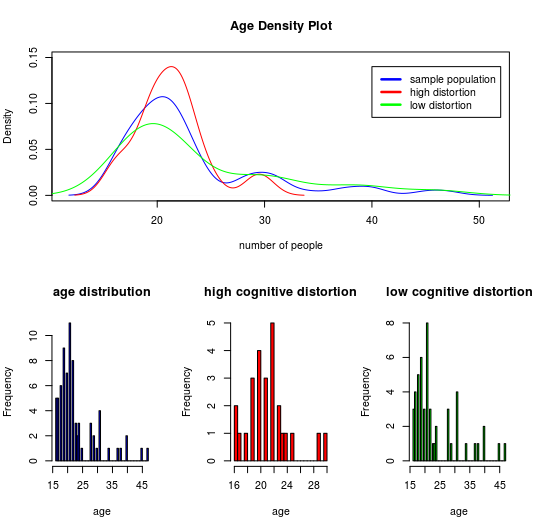
\includegraphics[width=80mm,scale=0.8]{fig2}
  \caption{Distribution of negative emotion and transdiagnostic symptoms}
  \label{fig:two}
\end{figure}


% Figure
\begin{figure}
  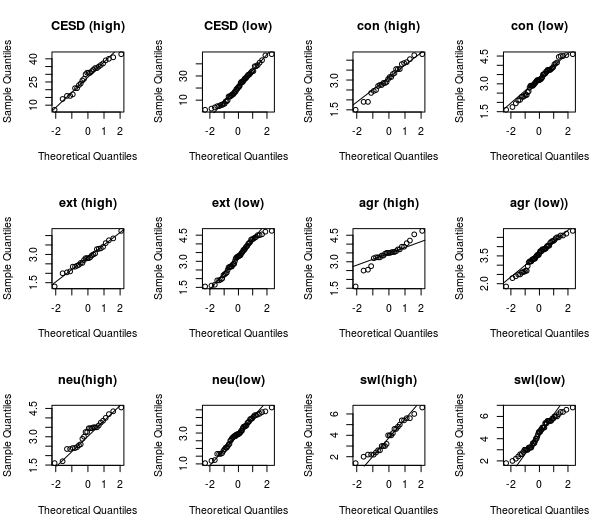
\includegraphics[scale=0.9]{CESD_distortion}
  \caption{qqplot of selected variables}
  \label{fig:three}
\end{figure}


% Table
\begin{table}%
\caption{t-test Between Users with High or Low Transdiagnostic Symptoms}
\label{tab:two}
\begin{minipage}{\columnwidth}
\begin{center}
\begin{tabular}{llllllllll}
  \toprule
        & \multicolumn{2}{c}{all(n=77)}	& \multicolumn{2}{c}{High Trans(n=26)}   & \multicolumn{2}{c}{Low Trans(n=29)} &  &  \\ 
   &  mean  & SD &  mean & SD &  mean & SD & p & Cohen's d \\     

  \hline\hline
  SWL  & 4.221 &  & 3.831 &  &4.483 &  &  & -0.42 \\
  CES-D  & 23.860 &  & 28.42 &  &21.62 &  & * & 0.60 \\
  ope  & 4.166 &  & 4.052 &  &4.148 &  &  &-0.37 \\
  con  & 3.183 &  & 3.085 &  &3.094 &  &  & -0.19\\
  ext  & 3.101 &  & 2.838 &  &3.094 &  &  & -0.48 \\
  agr  & 3.539 &  & 3.457 &  &3.522 &  &  &-0.18 \\
  neu  & 3.022 &  & 3.152 &  &2.96 &  &  & 0.22 \\

\bottomrule
\end{tabular}
\end{center}
\bigskip\centering

 \emph{Note:} * p<0.05, **p<0.01, ***p<0.001 after boferroni correction. Effect size: 0.8 = large(L);  0.5= moderate(M); 0.2 = small(S)
num. of posts: Number of posts in two months;  SWL: Satisfaction with Life score
CES-D: Center for Epidemiological Studies Depression (CESD); ope: openness; con: conscientiousness; ext: extraversion; agr: agreeableness;  neu: neuroticism. 

\end{minipage}
\end{table}%

We present transdiagnostic symptoms scores from the two groups together with their self-reported big-5 personality score, satisfaction with life score and depression symptom score Table ~\ref{tab:two} . Two users didn’t report their age on their profiles, here we assign the mean age to the them. We conduct independent sample t-tests on the selected variables among the two groups. Figure ~\ref{fig:three} shows the qqplot of the selected variables. 

Our observation indicate that users' personality characteristics does not distinguish their transdiagnostic symptoms. However, users with more transdiagnostic symptoms tend to post more posts (nearly twice more than the low symptom group).  They also reported significantly more depression symptoms (28\% higher than low symptom users).

We further divide users according to their demographic characteristics (gender, marital status, relationship status and relationship with parents), and observe their differences in transdiagnostic symptoms Table ~\ref{tab:three}. Users missing some of the characteristics information are assigned under the category 'other', users in this category are not included in this analysis. Since Figure \label{fig:two} shows that the transdiagnostic symptoms and negative emotion are not in normal distribution. We conduct Wilcoxon signed-rank test (non-parametric test used when the sample is not normally distributed) to compare these components between male and female. Result shows that there is no gender difference in transdiagnostic symptoms. 

We attempt to find out if relationship status contribute to the amount of transdiagnostic symptoms. We used Kruskal-Wallis test to compare the median between users with different relationship status: single, be in a relationship, married. Kruskal-Wallis test is a non-parametric equivalent of one-way analysis of variance (ANOVA). ANOVA is used when the residuals are normally distributed, which is not the case in our sample. Whereas, Kruskal-Wallis can be used to compare the median between the groups when this assumption is not satisfied. Result shows the three groups show no statistical significance in negative emotion (H= 4.516, p >0.05), cognitive distortion (H = 1.573, p >0.05) and negative thinking(H = 1.628, p >0.05). Although the median of the three groups appears no difference but the density plots from the three groups show that most of the married individuals have significantly lower transdiagnostic symptom and negative emotion \label{fig:three}. Having a partner to provide mental support seems to be a protective factor, whereas, no difference is found among people being in a relationship. Therefore, the result can be interpreted the other way around, people has a partner and with less transdiagnostic symptoms are more likely to get married or report married on social media. Moreover, individuals without divorced parents tend to have lower negative emotion cognitive distortion and negative thinking compared with those who have divorced parents. 

% Figure
\begin{figure}
  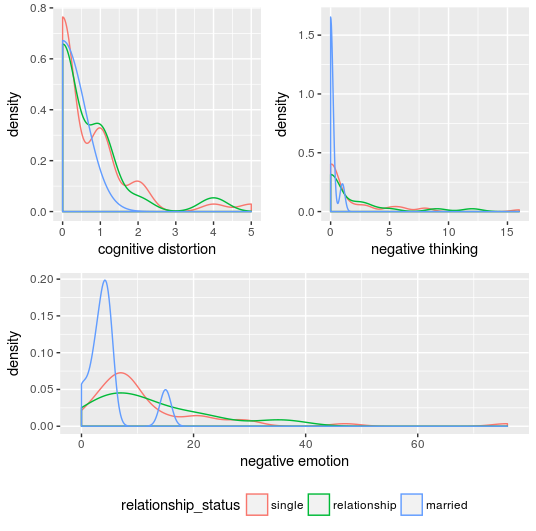
\includegraphics[scale=0.9]{neg_emo_rela}
  \caption{negative emotion in different relationship statuses}
  \label{fig:three}
\end{figure}


% Table
\begin{table}%
\caption{Comparing Transdiagnostic Symptoms Among Different Demographic Groups}
\label{tab:three}
\begin{minipage}{\columnwidth}
\begin{center}
\begin{tabular}{lllllllllll}
  \toprule
        & \multicolumn{2}{c}{parents together}	& \multicolumn{2}{c}{parents NOT together}     \\ 
      & mean &  SD & mean &  SD & p & Hodges-Lehmann estimator \\   
    \hline
    \hline
 Negative emotion  &6.315  & 4.607 & 13.292 &4.607 &* & -0.067 \\
  Cognitive distortion   &0.158  & 0.374 &0.625 &1.095 & &0.000 \\
  Negative thinking  &0.263  & 0.653 & 1.75 &2.937 & &0.000\\
  CES-D  &19.63  & 10.24 & 25.12 &12.74 & & 6.000\\
  \bottomrule
\end{tabular}
\end{center}
\bigskip\centering

 \emph{Note:} * p<0.05, **p<0.01, ***p<0.001. Hodges-Lehmann test estimates the pseudo-median in non-parametric test. Hodges-Lehmann estimator shows the difference between the pseudo-median.

\end{minipage}
\end{table}%


% Head 3
\subsection{Late night posts}
Sleep disturbance is one of the major symptoms in depression. We investigate the relationship between sleep disturbance and cognitive distortion. We count the number of posts written from midnight 12:00am until 6:00am in the morning. Then compute the proportion of late night post to the total number of post of that user. We investigate the relationship between proportion of late night post to transdiagnositic symptoms. For transdiagnositic symptoms, we divide the cumulative symptom by the number of post of the user.

Negative emotion  (r = 0.293, p < 0.01), cognitive distortion (r = 0.300, p < 0.01) and negative thinking (r = 0.285, p <0.05) are slightly correlated with number of late night post. It appears that negative thinking is more likely to occur in late night post. Our result is also supported by the cognitive model of insomnia. Insomnia individuals suffer unpleasant thoughts and excessive, uncontrollable worry during the pre-sleep period (Borkovec 1979, 1982; Morin, 1993). 

% Head 4
\subsection{Linguistics styles}
We also measure the correlation between transdiagnostic components and linguistics style. Linguistics styles capture how an individual use different components of the language in various psychological or social environments. We used LIWC to define the linguistics styles of each Facebook posts, then we aggregate the linguistic style score on user level. Table ~\ref{tab:four} shows the correlation between user linguistics style score and transdiagnostic symptoms. 

Clout refers to the social status, confidence, or leadership that people display through their writing. Study found that people with higher status tend to use less first-person pronoun and use more first-person plural and second-person singular pronoun \cite{Kacewicz13}. It appears in our result that clout is strongly correlated with people with more negative emotions. They tend to focus on self, thus, they use less 3rd person or 2ed person pronouns. Our finding is in correspond to the finding from Pennenaker's depression and language study \cite{Pennebaker10}. The difference of self-focus might be a result in response to emotional pain or a thinking pattern that is a predilection for depression \cite{Wolf07}.

It is not surprised to see that emotional tone, which refers to the positive tone, is negatively correlated with negative emotion score. Negative emotion is also moderately correlated with our manual labeled negative emotion. Social referents, which refers to words indicating social roles (father, mother, sister and so on) are slightly to moderately linked to cognitive distortion and negative emotion. Our result indicates that people shows more negative emotion and cognitive distortion on social media are more likely to be socially detached from family and friends.  We also find that these people are more present and future oriented and use less exclamation marks. However, this might be particular to social media text, because users seldom describe the negative events happen in the past with detail on Facebook posts, instead, they vent out their feelings to the events. For example, 'I am bored.' 'feeling sick again.' 'I hate today.' Exclamation marks is often used to indicate excitement or surprise in a positive context.

It appears that the content of negative thinking is often related to health and home. However, our result is limited to the context of social media, it's likely that people are less open to talk about financial situation and work issues on social media because that could affect their social image. On the other hand, posts that contain cognitive distortion is not content specific, they tend to have longer words and more words in a sentence and these words are more likely to be in the LIWC dictionary. This is mainly due to the fact that there is a lot of reasoning and thinking process in cognitive distortion posts. In addition, the language on cognitive distortion is also less reward focus and more risk or prevention focus.

% Table
\begin{table}%
\caption{Transdiagnositc components and depression symptoms}
\label{tab:four}
\begin{minipage}{\columnwidth}
\begin{center}
\begin{tabular}{llll}
  \toprule
           & Negative emotion & Cognitive distortion  & Negative thinking  \\ 
  \hline\hline
  SUMMARY VARIABLE   \\
  analytic &  & -0.262* &   \\
  clout & -0.518** &   &-0.310**   \\
  authentic &  & 0.325**  &   \\
  emotional tone & -0.341*** &   &   \\
  LANGUAGE MATRICS &  &   &   \\
  words > 6 letters &  & -0.335**  &   \\
  words per sentence &  & 0.258*  &   \\
  dictionary words & 0.234* & 0.412***  &   \\
  GRAMMAR &  &   &   \\
  functional words &  & 0.344**  &   \\
  total pronouns &  & 0.251**  &   \\
  personal pronouns &  & 0.251**  &   \\
  1st per pronoun & 0.369** & 0.325**  & 0.239*  \\
  3rd per singular &-0.326*& -0.249* &    \\
  2nd person & -0.235* &   &   \\
  prepositions &  & 0.273*  &   \\
  conjunctions &0.322**  & 0.309*  &   \\
  adjective &  & 0.270*  &   \\
  comparatives &  & 0.320**  &   \\
  verb & 0.244* &   &   \\
  AFFECT WORDS &  &   &   \\
  negative emotion &0.322**  &   &   \\
  anger &0.413***  &   &   \\
  anxiety &  &   &   \\
  sadness &  &   &   \\
  swear & 0.385*** &   &   \\
  SOCIAL  &  &   &   \\
  social words &  &   & -0.263*  \\
  female referents &-0.338** & -0.237* &     \\
  male referents &  & -0.261*  &   \\
  COGNITIVE PROCESS &  &   &   \\
  differentiation &0.323**  &   &   \\
  PERCEPTUAL &  &   &   \\
  perceptual process &  &0.255*   &   \\
  feeling &  & 0.301*  &   \\
  BIOLOGICAL &  &   &   \\
  health/illness &  &   & 0.335*  \\
  CORE DRIVE &  &   &   \\
  reward focus &  & -0.249*  &   \\
  risk/prevention focus &  & 0.312**  &   \\
  TIME &  &   &   \\
  present focus & 0.247* & 0.232*  &   \\
  future focus &0.312*  &   &   \\
  PERSONAL CONCERN &  &   &   \\
  home & 0.300** &   &   0.246*\\
  work &  &   &   \\
  money &  &   &   \\
  PUNCTUATION &  &   &   \\
  exclamation marks &-0.257*  &-0.317*   &   \\
  


  \bottomrule
\end{tabular}
\end{center}
\bigskip\centering

 \emph{Note:} * p<0.05, **p<0.01, ***p<0.001 

\end{minipage}
\end{table}%

% Head 4
\subsection{Cognitive Distortion Regression Model}

We explore the performance of a linear regression model in predicting cognitive distortion. We found high interactions between the LIWC features. Whereas, PCA or SVD-based feature selection methods do not take into account the potential multivariate nature of the data structure. We select features that are most correlated with cognitive distortion according to Table~\ref{tab:four}. "Dictionary words" has the highest correlation with cognitive distortion but also has high interaction with more 1/3 of the language features, therefore, we removed "dictionary words" to avoid multivariation. Then we further remove features that are more than 0.3 correlated with the top features. Our model explains 52\% of variance in the data. Swear words and Risk focus are very strong predictors.

% Table
\begin{table}%
\caption{Cognitive Distortion Linear Regression Model}
\label{tab:five}
\begin{minipage}{\columnwidth}
\begin{center}
\begin{tabular}{lllll}
  \toprule
        measures & beta	& SE   & t-Stat \\
  \hline
  \hline 
Intercept        &   0.199  &0.160 &  1.240  \\ 
total pronouns&  0.010* &  0.004 &  2.221 \\
3rd person pronoun  & -0.019*  & 0.008 & -2.291   \\
preposition   &  0.021**  & 0.007 &  2.837  \\
swear  &  0.021***  & 0.005 &  4.026\\
feeling   &  0.029**  & 0.010 &  2.929  \\
reward focus & -0.020*  & 0.009 & -2.132 \\
risk focus   &  0.030***  & 0.008 &  3.494 \\
proportion of late night post        &   1.031*  & 0.426 &  2.417 \\

  \hline
  Residual standard error &  0.714  \\
  Multiple-R2 &  0.521 \\ 
  Error degrees of freedom  & 68  \\ 
  \hline
  \bottomrule
\end{tabular}
\end{center}
\bigskip\centering

 \emph{Note:} . < 0.1 * p<0.05, **p<0.01, ***p<0.001 
parents not together1: no and not in contact with mother; parents not together2: no but in frequent contact with parents; 

\end{minipage}
\end{table}%

\section{CONCLUSION}
This research is designed as an approach to complement the current transdiagnositic diagnostic approach with a novel way to access people's behavior. We examine the feasibility to identify transdiagnostic symptoms using Facebook data and finding out the language features that are able to predict cognitive distortion, a core component in CBT, which is highly associated with anxiety and depressive disorders. First, we label negative emotion, cognitive distortion and negative thinking in more than 4000 Facebook posts. Then we investigate the relationship between these components and depression symptoms, satisfaction with life and big-5 personality. Thereafter, we characterize the differences of transdiagnostic symptoms and negative emotions among different demographic groups. Finally, we identify features that are able to predict cognitive distortion.

We found that cognitive distortion is moderately correlated with depression symptoms and satisfaction with life. Marriage and without divorced parents seem to be protective factors in developing transdiagnostic symptoms. We found that some of the language features are best predicting cognitive distortion (explained 55\% of variance in the data). The proportion of posts written at mid night, which is a sign of insomnia, also enhance the prediction. 

The major limitation of our work is that our data is from social media platform. Facebook data may not represent the thinking process of an individual most precisely, because users have different degree of selective biased presentation and self-disclosure level. Moreover, this work focus on a limited set of sample that involve 77 users. It would be useful to replicate the study on a larger population to validate the pattern we found in here. 




